\subsection{Idea general del problema}
Se nos propone realizar un algoritmo en el que dados n número enteros en cualquier orden se debe devolver otros n números, donde el i-ésimo de ellos represente la parte entera de la mediana de los primeros i números de la entrada.
La mediana de un conjunto ordenado de n números se define como x$_{(n+1)/2}$ si n es impar, o como (x$_{n/2}$ + x$_{n/2+1)}$)/2  si n es par.
Un ejemplo de entrada puede ser \\
2 7 2 8 4 9 1 6 5
y su salida deberia ser \\
2 4 2 4 4 5 4 5 5
\subsection{Explicación, correctitud y pseudocódigo}

Lo que hicimos fue dividir un arreglo (L) de tamaño n en dos conjuntos (multiconjuntos, ie: pueden tener repetidos), uno con los elementos menores a cierto número (A) y otro con los mayores (B). Los elementos iguales a ese número pueden ir en cualquiera de los dos. Entonces sabemos que, si ordenaramos el arreglo, L[ \textbar A\textbar] = max(A) y L[\textbar A\textbar+1] = min(B). Tres casos importantes: 

\begin{itemize}
\item Si ambos conjuntos tienen la misma cantidad de elementos entonces L[\textbar A\textbar] = L[n/2] = max(A) y L[n/2+1] = min(B). Entonces la mediana(L) = (max(A)+min(B))/2
\item Si \textbar A\textbar = \textbar B\textbar + 1 (n es impar), entonces L[(n+1)/2] = max(A). Entonces la mediana(L) = max(A)
\item Si \textbar A\textbar + 1 = \textbar B\textbar (n es impar), entonces L[(n+1)/2] = min(B). Entonces la mediana(L) = min(B)
\end{itemize}


Nuestro algoritmo lo que hace es: 
\begin{itemize}
\item Si el arreglo original no contiene elementos, entonces devolvemos un vector vacio
\item Insertar el primer elemento en el conjunto de los elementos más grandes (B) e insertarlo también en la posición 1 del resultado, ya que es mediana.
\item Hasta que no queden elementos en el arreglo original, se agrega el elemento i del arreglo original en el conjunto A si es menor a la mediana del paso anterior y al conjunto B si es mayor. Si la diferencia entre la cantidad de elementos de ambos conjuntos es igual a 2, entonces quitamos el mayor elemento de A o el menor elemento de B y lo insertamos en el otro para que nos queden dos conjuntos de igual tamaño. Entonces podemos utilizar la propiedad de arriba y sacar fácilmente la mediana, obteniendo el máximo y/o mínimo de los conjuntos correspondientes. Ponemos la mediana en la posición i del resultado y avanzamos a la siguiente iteración.
\end{itemize}

A continuación mostraremos su pseudocódigo y deduciremos su complejidad: \\
--------------------------------------------------------------------------------------------------------------\\
vector$<$int$>$ medianas(vector$<$int$>$ a)\{ \\
$~~~~~~~~~~~~~$\textbf{si} (a es vacio) \{ \\ \IfOde{1}\\
$~~~~~~~~~~~~~~~~~~$devolvemos un vector vacio \Ode{1}\\
$~~~~~~~~$\} \\
$~~~~~~~~$creamos el vector res de tamaño igual que a, inicializado con ceros\Ode{tamaño de a} \\
$~~~~~~~~$res[0] $\leftarrow$ a[0]\Ode{1} \\
$~~~~~~~~$creamos el multiset vacío: masGrandes \Ode{1} \\
$~~~~~~~~$creamos el multiset vacío: masChicos \Ode{1} \\
$~~~~~~~~$int mínimo\Ode{1} \\
$~~~~~~~~$int máximo\Ode{1} \\
$~~~~~~~~$insertamos a masGrandes el primer elemento del vector \Ode{log(tamaño de masGrandes)} = \Ode{1} \\
$~~~~~~~~$ \textbf{para cada} (int i = 1; i $<$ al tamaño de a; i++)\{ \\ \WhileOdeb{tamaño de a} \\
$~~~~~~~~~~~~~$\textbf{si} (el elemento i de a $\geq$ el elemento i-1 de res)\{ \\ \IfOde{1} \\
$~~~~~~~~~~~~~~~~~~$insertamos a masGrandes el elemento i de a \Ode{log(tamaño de masGrandes)} \\
$~~~~~~~~~~~~~$ \} \textbf{si no} \{ \\
$~~~~~~~~~~~~~~~~~~$ lo insertamos en masChicos \Ode{log(tamaño de masChicos)} \\
$~~~~~~~~~~~~~$ \} \\
$~~~~~~~~~~~~~$\textbf{si} (el tamaño de masGrandes - tamaño de masChicos == 2) \{ \\ \IfOde{1}\\
$~~~~~~~~~~~~~~~~~~$minimo $\leftarrow$ $\ast$ masGrandes.begin() \Ode{1}\\
$~~~~~~~~~~~~~~~~~~$borramos mínimo de masGrandes  \Ode{log(tamaño de masGrandes)} \\
$~~~~~~~~~~~~~~~~~~$insertamos minimo a masChicos \Ode{log(tamaño de masChicos)} \\
$~~~~~~~~~~~~~$\} \textbf{si no, si}(el tamaño de masGrandes - tamaño de masChicos == -2) \{ \\ \IfOde{1}\\
$~~~~~~~~~~~~~~~~~~$maximo $\leftarrow$ $\ast$ masChicos.rbegin() \Ode{1}\\
$~~~~~~~~~~~~~~~~~~$borramos máximo de masChicos \Ode{log(tamaño de masChicos)} \\
$~~~~~~~~~~~~~~~~~~$insertamos máximo a masGrandes \Ode{log(tamaño de masGrandes)} \\
$~~~~~~~~~~~~~$\} \\
$~~~~~~~~~~~~~$\textbf{si} (el tamaño de masGrandes == el tamaño de masChicos) \{ \\ \IfOde{1}\\
$~~~~~~~~~~~~~~~~~~$minimo $\leftarrow$ $\ast$ masGrandes.begin() \Ode{1}\\
$~~~~~~~~~~~~~~~~~~$maximo $\leftarrow$ $\ast$ masChicos.rbegin() \Ode{1}\\
$~~~~~~~~~~~~~~~~~~$posicion i de res $\leftarrow$ (maximo + minimo)/2; \Ode{1}\\
$~~~~~~~~~~~~~$\} \textbf{si no, si} (el tamaño de masGrandes - el tamaño de masChicos == 1) \{ \\ \IfOde{1}\\
$~~~~~~~~~~~~~~~~~~$minimo $\leftarrow$ $\ast$ masGrandes.begin() \Ode{1} \\
$~~~~~~~~~~~~~~~~~~$posición i de res $\leftarrow$  minimo \Ode{1} \\
$~~~~~~~~~~~~~$\} \textbf{si no, si} (el tamaño de masGrandes - tamaño de masChicos == -1) \{ \\ \IfOde{1}\\
$~~~~~~~~~~~~~~~~~~$maximo $\leftarrow$ $\ast$ masChicos.rbegin() \Ode{1}\\
$~~~~~~~~~~~~~~~~~~$posición i de res $\leftarrow$ maximo \Ode{1}\\
$~~~~~~~~~~~~~$\} \\
$~~~~~~~~$\} \\
$~~~~~~~~$devolvemos res \Ode{1}\\
\} \\
------------------------------------------------------------------------------------------------------------\\

\subsection{Deducción de la cota de complejidad temporal}
Los conjuntos utilizados son  \textbf{$<$multiset$>$} cortesía de C++. La inserción y borrado cuesta O(log(n)) siendo n la cantidad de elementos del conjunto, ya que usamos las funciones de C++: \textbf{insert} y \textbf{erase} de los \textbf{multisets}, respectivamente. La función \textbf{erase} cuesta O(log(n)) + O(m) siendo n = cantidad de elementos del conjunto, y m el número de elementos eliminados, en nuestro caso, siempre es uno porque llamamos a erase una vez con el elemento mínimo y otra con el máximo.\\
Obtener máximo y mínimo nos cuesta O(1), pues usamos \textbf{begin()} y \textbf{rbegin()} de complejidad constante. Además usamos la función \textbf{size} de los \textbf{multisets} de complejidad constante. \\ 

Tenemos como entrada un vector de tamaño n. Los pasos a realizar son: \\

1) Crear el vector donde se guardará y devolverá el resultado: se realiza en O(n). \\

2) Insertar el primer elemento del arreglo original en el arreglo resultado es O(1), porque usamos \textbf{operator[]} de complejidad constante. \\

3) Luego, se realizan n-1 iteraciones, en las cuales: \\
\begin{itemize}
\item Se realiza una comparación O(1) y se hace una inserción en alguno de los conjuntos en O(log(n)).
\item Si la diferencia entre la cantidad de elementos de ambos conjuntos es igual a 2, se elimina el mayor elemento de A o el menor elemento de B en O(log(n)) y lo insertamos en el otro en O(log(n)).
\item Obtenemos el máximo y/o mínimo de los conjuntos correspondientes para calcular la mediana y la insertamos en el resultado en O(1).
\end{itemize}
Aclaración: en este ciclo, en realidad, las complejidades no son O(log(n)) sino que son O(log(i)) siendo i el número de iteración. Pero como i $<$ n $\forall$ i, entonces lo acotamos por O(log(n)). \\

Entonces la complejidad total del algoritmo es O(n + (n-1)log(n)) = O(n log(n)).

\subsection{Casos de test y sus gráficos}
Vamos a analizar los tiempos de nuestro algoritmo para entradas de distinto tamaño, divididos en tres casos (todos O(n log n)):
\begin{itemize}
\item Peor caso: Corresponde al caso donde en la mitad de las iteraciones del ciclo, la diferecia entre la cantidad de elementos entre los conjuntos masGrandes y masChicos es igual a dos. Entonces hay que realizar en cada una de estas un borrado y una insercion. No existe peor caso que este, ya que al realizar una insercion y borrado, los conjuntos quedan con la misma cantidad de elementos y se necesitan dos iteraciones mas ciclo para tener que volver a reacomodar los elementos. Entradas crecientes y decrecientes son ejemplos de peor caso, que es lo que utilizaremos
\item Mejor caso: Resulta cuando en ninguna iteracion la diferecia entre la cantidad de elementos entre los dos conjuntos es igual a dos, y no hay que hacer borrado e insercion. Para que pase esto, nuestra entrada consistira en una cadena de numeros, donde la subcadena de numeros en posicion par es creciente, y la subacadena de numeros en posicion impar es decreciente 
\item Caso random: Utilizando la funcion random de python, generamos entradas al azar de diferentes entradas
\end{itemize}

\begin{figure}[H]
\begin{center}

\minipage{0.8\textwidth}
  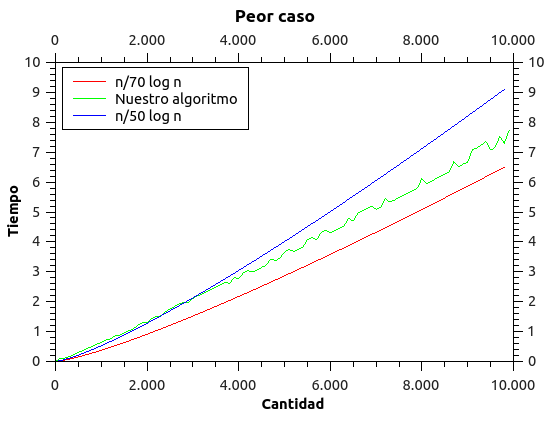
\includegraphics[width=\linewidth]{../graficos/ej2/Peor.png}
  \caption{{\small Comparación del peor caso con O((n/6000)log(n)) y O((n/4200)log(n)).}} \label{ej2-peor-caso}
\endminipage

\end{center}
\end{figure}


\begin{figure}[H]
\begin{center}

\minipage{0.8\textwidth}
  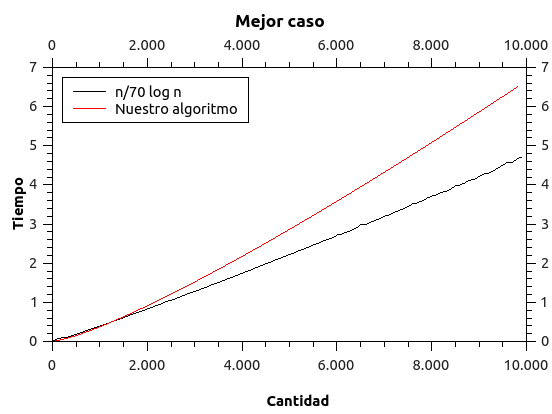
\includegraphics[width=\linewidth]{../graficos/ej2/Mejor.png}
  \caption{{\small Comparación del mejor caso con O((n/6000)log(n)).}} \label{ej2-mejor-caso}
\endminipage

\end{center}
\end{figure}


\begin{figure}[H]
\begin{center}

\minipage{0.8\textwidth}
  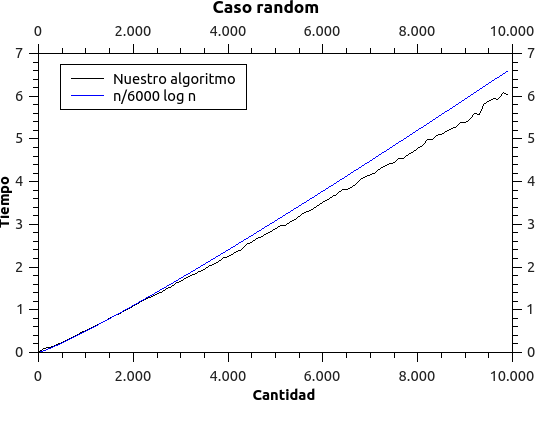
\includegraphics[width=\linewidth]{../graficos/ej2/Random.png}
  \caption{{\small Comparación de un caso random con O((n/6000)log(n)).}} \label{ej2-random-caso}
\endminipage

\end{center}
\end{figure}

\begin{figure}[H]
\begin{center}

\minipage{0.8\textwidth}
  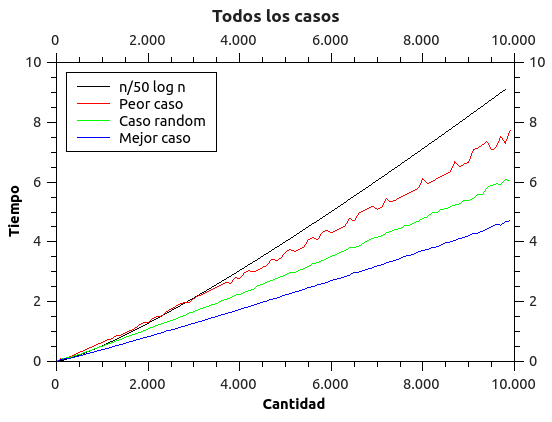
\includegraphics[width=\linewidth]{../graficos/ej2/Todos.png}
  \caption{{\small Comparación de los tres casos anteriores con O((n/5000)log(n)).}} \label{ej2-todos-casos}
\endminipage

\end{center}
\end{figure}
